% ============================================================================
% Staged Calibration of Tensor-Basis Turbulence Closures:
% Transient Realizability Dynamics in Nested Subspaces
% ============================================================================
\documentclass[preprint,aps,prb,longbibliography,superscriptaddress]{revtex4-2}

\usepackage{amsmath,amssymb,amsthm}
\usepackage{booktabs}
\usepackage{graphicx}
\usepackage{siunitx}
\usepackage{tikz}
\usetikzlibrary{arrows.meta,positioning,calc}
\usepackage{xcolor}
\usepackage{hyperref}
\usepackage{multirow}

\hypersetup{
  colorlinks=true,
  linkcolor=blue!60!black,
  citecolor=blue!60!black,
  urlcolor=blue!60!black,
}

% --- Custom commands ---
\newcommand{\bx}{\mathbf{x}}
\newcommand{\bU}{\mathbf{U}}
\newcommand{\bI}{\mathbf{I}}
\newcommand{\Tr}{\operatorname{Tr}}
\newcommand{\dR}{\delta_R}
\newcommand{\fsec}{f_{\text{sec}}}
\newcommand{\tref}{\tau_{\text{ref}}}

\begin{document}

% ============================================================================
\title{Staged Calibration of Tensor-Basis Turbulence Closures:\\
Transient Realizability Dynamics in Nested Subspaces}

\author{Okuhle Madondo}
\affiliation{Department of Mechanical Engineering / Machine Learning Research Group}
\email{okuhlemadondo@users.noreply.github.com}

\date{\today}

% ============================================================================
\begin{abstract}
Data-driven turbulence closure modeling requires navigating a space of
candidate model structures (discrete tensor basis selections) and continuous
scalar coefficients. In a controlled \emph{a~priori} study of
constant-coefficient Pope tensor-basis closures on a synthetic square duct
benchmark ($\mathrm{Re}_\tau = 300$), we investigate whether staging
calibration through intermediate subspaces---calibrating a quadratic
truncation before extending to cubic---offers measurable advantages over
direct joint calibration.

We find that staging relocates transient realizability violations into a
non-deployed scaffold stratum, yielding essentially monotone repair dynamics
upon deployment into the full parameter space. Through a $2\times 2$ ablation
matrix crossing basis scaling (raw vs.\ unit-normalized) with optimizer choice
(Adam vs.\ plain gradient descent), we identify the mechanism driving direct
calibration's transient instability: Adam's adaptive momentum interacting with
the realizability penalty barrier, not Gram matrix ill-conditioning. Plain
gradient descent produces zero realizability violations regardless of basis
scaling.

A cold-start baseline ($\theta = \mathbf{0}$) converges to the same final
loss as both warm-started paths with lower peak violation
($1.22\%$ vs.\ $2.00\%$ for direct warm-start), demonstrating that
warm-starting's advantage in this convex setting is limited to trajectory
quality under momentum-based optimizers, not to convergence speed or endpoint
accuracy. We frame these findings within a \emph{Stratified Design Atlas}
formalism that organizes model families as nested subspaces connected by
zero-padding embeddings, and outline the theoretical horizon for non-nested
structural edits where learned transport maps and non-convex losses make
path-dependence genuinely geometric.
\end{abstract}

\maketitle

% ============================================================================
\section{Introduction}\label{sec:intro}
% ============================================================================

Turbulence closure modeling for Reynolds-Averaged Navier--Stokes (RANS)
equations remains one of the foundational open challenges in computational
fluid dynamics. The Reynolds stress tensor
$\tau_{ij} = \overline{u_i' u_j'}$ represents the statistical effect of
turbulent fluctuations on the mean momentum field. For decades, practical
engineering CFD has relied on linear eddy-viscosity models governed by the
Boussinesq hypothesis~\cite{Boussinesq1877}:
\begin{equation}\label{eq:boussinesq}
  \tau_{ij} - \tfrac{2}{3}k\,\delta_{ij} = -2\,\nu_t\, S_{ij}\,,
\end{equation}
where $k$ is the turbulent kinetic energy, $\nu_t$ is the scalar eddy
viscosity, and $S_{ij} = \tfrac{1}{2}(\partial_j U_i + \partial_i U_j)$ is
the mean strain rate tensor.

While computationally robust, the Boussinesq hypothesis fails qualitatively in
complex strain fields---most notoriously in non-circular duct flows, where
turbulent secondary motion of the second kind~\cite{Prandtl1926} is driven
predominantly by Reynolds normal stress anisotropy
$(\tau_{yy} - \tau_{zz})$ and cross-stream shear stress
$\tau_{yz}$~\cite{Speziale1987}. Linear models produce secondary vorticity
forcing that is anti-aligned with the physical forcing pattern, a classical
result due to Speziale~\cite{Speziale1987}.

To overcome these deficiencies, higher-order non-linear eddy viscosity models
\cite{Pope1975,Craft1996,Wallin2000} have been developed. Modern automated
model discovery frameworks face a practical challenge when navigating this
space of candidate models:
\begin{itemize}
  \item \textit{Cold-start cost.} Re-optimizing all continuous parameters from
    scratch each time a structural modification is made (adding, removing, or
    swapping tensor basis terms) discards prior calibration work.
  \item \textit{Warm-starting risks.} Initializing new coefficients to zero
    (or other heuristic values) preserves the prior calibration by
    construction, but the subsequent optimization trajectory may interact
    adversely with physical constraints such as
    realizability~\cite{Schumann1977,Lumley1978}.
\end{itemize}

\subsection{Approach and Scope}\label{sec:scope}

We formalize the space of nested tensor-basis closures as a collection of
coordinate subspaces connected by zero-padding embeddings, which we term a
\emph{Stratified Design Atlas}. In this simplest instantiation---nested
constant-coefficient Pope subspaces with a convex quadratic task
loss---zero-padding is exact by construction ($\dR \equiv 0$), endpoint
agreement is guaranteed by convexity, and the geometric vocabulary (atlases,
connections, curvature) names structure that is trivial. The framework's value
lies in organizing the design space for future extensions to non-nested edits
and non-convex losses (Sec.~\ref{sec:discussion}), where these structures
become non-trivial.

The contribution of this paper is a controlled \emph{a~priori} study of the
\emph{transient dynamics} of warm-started calibration under realizability
constraints:
\begin{enumerate}
  \item We quantify the stress-representability gap between linear and
    quadratic Pope strata, recovering the classical
    result~\cite{Speziale1987} that linear closures produce anti-aligned
    secondary vorticity forcing.
  \item We demonstrate that staging calibration through intermediate subspaces
    relocates transient realizability violations into a non-deployed scaffold
    model, yielding smoother deployment dynamics at the cost of a larger but
    discarded scaffold violation.
  \item Through a $2\times 2$ ablation matrix, we identify the transient
    instability mechanism as Adam momentum interacting with the penalty
    barrier, not Gram matrix ill-conditioning.
  \item A cold-start baseline contextualizes the warm-starting advantage:
    it converges to the same endpoint with lower peak violation, showing that
    the staging benefit is specific to momentum-based optimizers.
\end{enumerate}

% ============================================================================
\section{Mathematical Formulation}\label{sec:math}
% ============================================================================

\subsection{Governing Equations and Secondary Flow Mechanics}
\label{sec:governing}

Consider steady, incompressible turbulent flow through a straight square duct
of width $h$ aligned with the $x$-axis. The mean velocity field is
$\bU = (U(y,z),\, V(y,z),\, W(y,z))$, which is $x$-independent but
three-dimensional: $\partial U/\partial y$, $\partial U/\partial z \neq 0$,
and the secondary velocities $(V,W)$ are nonzero. Defining the streamwise
mean vorticity
\begin{equation}
  \omega_x = \frac{\partial W}{\partial y} - \frac{\partial V}{\partial z}\,,
\end{equation}
the secondary vorticity driving force $\fsec$ is defined by
spatial derivatives of the Reynolds stresses:
\begin{equation}\label{eq:fsec}
  \fsec(\bx) =
  \underbrace{\frac{\partial^2}{\partial y\,\partial z}
    (\tau_{yy} - \tau_{zz})}_{\text{Normal stress anisotropy}}
  +\;
  \underbrace{\left(\frac{\partial^2}{\partial z^2}
    - \frac{\partial^2}{\partial y^2}\right)\tau_{yz}}_{\text{Cross-plane shear stress}}\,.
\end{equation}

\subsection{Tensor Integrity Basis and Nested Subspaces}
\label{sec:basis}

Following Pope~\cite{Pope1975}, the deviatoric Reynolds stress anisotropy
$a_{ij} = \tau_{ij}/k - \tfrac{2}{3}\delta_{ij}$ can be expanded in a
complete integrity basis of the non-dimensional symmetric strain rate
$S_{ij}^*$ and anti-symmetric rotation rate $\Omega_{ij}^*$:
\begin{equation}\label{eq:pope_expansion}
  a_{ij} = \sum_{n=1}^{N} c_n(\bI)\, T_{ij}^{(n)}\,.
\end{equation}
In the square duct, the mean velocity field is $x$-independent but has
three-dimensional strain via $\partial U/\partial y$ and
$\partial U/\partial z$. We \emph{select} (not truncate) four tensors from
Pope's ten-term basis to form three nested subspaces. The strata defined here
use \emph{spatially constant} coefficients $\theta$, corresponding to
constant-coefficient truncations of Pope's general expansion.

\paragraph{Stratum~0 ($\mathcal{M}_0$, Linear Boussinesq, $d_0 = 1$).}
\begin{equation}\label{eq:stratum0}
  \tau^{(0)}(\bx;\theta) = \tfrac{2}{3}k\,I + \theta_0\, T^{(1)},
  \qquad
  T^{(1)} = -\frac{2k}{\omega}\, S\,,
\end{equation}
where $\theta_0 = C_\mu \approx 0.09$.

\paragraph{Stratum~1 ($\mathcal{M}_1$, Quadratic, $d_1 = 3$).}
\begin{equation}\label{eq:stratum1}
  \tau^{(1)}(\bx;\theta) = \tfrac{2}{3}k\,I
  + \theta_0\, T^{(1)}
  + \theta_1\, T^{(2)}
  + \theta_2\, T^{(3)}\,,
\end{equation}
with
\begin{equation}\label{eq:T2T3}
  T^{(2)} = \frac{k}{(C_\mu\omega)^2}
    \Bigl(S^2 - \tfrac{1}{3}\Tr(S^2)\,I\Bigr),
  \quad
  T^{(3)} = \frac{k}{(C_\mu\omega)^2}
    \bigl(S\Omega - \Omega S\bigr).
\end{equation}

\paragraph{Stratum~2 ($\mathcal{M}_2$, Cubic, $d_2 = 4$).}
\begin{equation}\label{eq:stratum2}
  \tau^{(2)}(\bx;\theta) = \tfrac{2}{3}k\,I
  + \sum_{i=0}^{3} \theta_i\, T^{(i+1)}\,,
\end{equation}
where $T^{(4)}$ is a cubic invariant tensor:
\begin{equation}\label{eq:T4}
  T^{(4)} = \frac{k}{(C_\mu\omega)^3}
    \bigl(S^2\Omega - \Omega S^2\bigr).
\end{equation}

\subsection{Stress-Representability Metrics}
\label{sec:representability}

To quantify whether a subspace can represent the secondary flow driving
stress, we define two distinct metrics.

The \emph{stress-projection alignment} $\cos\phi_{\mathrm{sec}}$ measures
whether the secondary stress pattern $\tau_{\mathrm{sec}}$ (the
$(\tau_{yy}-\tau_{zz})$ and $\tau_{yz}$ components of $\tref$) lies in the
$L^2(\Omega)$ span of the basis tensors:
\begin{equation}\label{eq:controllability}
  \cos\phi_{\mathrm{sec}}(\mathcal{M}_s) =
  \frac{\langle \tau_{\mathrm{sec}},\;
        \mathrm{proj}_{\mathcal{M}_s}\tau_{\mathrm{sec}}
        \rangle_{L^2(\Omega)}}
       {\|\tau_{\mathrm{sec}}\|_{L^2}\;
        \|\mathrm{proj}_{\mathcal{M}_s}\tau_{\mathrm{sec}}\|_{L^2}}\,.
\end{equation}

The \emph{forcing correlation} $\rho$ measures the alignment of the secondary
vorticity forcing field (Eq.~\ref{eq:fsec}) produced by a specific model
$\tau(\theta)$ with the reference forcing:
\begin{equation}\label{eq:rho}
  \rho(\theta) =
  \frac{\langle \fsec(\tau(\theta)),\;
        \fsec(\tref) \rangle_{L^2(\Omega)}}
       {\|\fsec(\tau(\theta))\|_{L^2}\;
        \|\fsec(\tref)\|_{L^2}}\,.
\end{equation}
These metrics measure different things: $\cos\phi_{\mathrm{sec}}$ is an
existence statement about the basis span (independent of $\theta$), while
$\rho$ evaluates the vorticity forcing at a specific $\theta$ and involves
second spatial derivatives.

\subsection{Zero-Padding Embeddings and Loss Landscape}
\label{sec:embedding}

For the nested inclusions $\mathcal{M}_0 \subset \mathcal{M}_1 \subset
\mathcal{M}_2$, zero-padding defines the embedding:
\begin{equation}\label{eq:transport}
  T_e(\theta) = \bigl[\theta_0,\, \theta_1,\, \dotsc,\,
    \theta_{d_s-1},\,
    \underbrace{0,\, \dotsc,\, 0}_{d_{s'}-d_s}\bigr].
\end{equation}
For any model family linear in $\theta$, zero-padding preserves predictions
identically:
$\tau^{(s')}(T_e(\theta)) = \tau^{(s)}(\theta)$ pointwise, so the realization
drift $\dR \equiv 0$ by construction. We verify this numerically.

Because $\tau$ is affine in $\theta$, the task loss
$L_{\text{task}}(\theta) = \tfrac{1}{2}\int_\Omega
\|\tau(\theta) - \tref\|_F^2\,dA$ is quadratic with constant Hessian equal to
the spatial \emph{Gram matrix}:
\begin{equation}\label{eq:gram}
  G_{ij} = \int_\Omega \Tr\bigl(T^{(i)}(\bx)\, T^{(j)}(\bx)\bigr)\,dA\,.
\end{equation}

To enforce physical validity, a realizability penalty is added:
\begin{equation}\label{eq:penalty}
  L(\theta) = L_{\text{task}}(\theta)
  + \lambda_{\mathrm{realiz}}
    \int_\Omega \max\!\bigl(0,\, -\lambda_{\min}(\tau(\bx;\theta))\bigr)^2\,dA\,,
\end{equation}
where $\lambda_{\min}$ denotes the smallest eigenvalue of the local stress
tensor. Since $\tau$ is affine in $\theta$ and the penalty is convex
(composition of convex nondecreasing $\max(0,\cdot)^2$ with concave
$-\lambda_{\min}$), the full loss $L(\theta)$ is convex when $G \succ 0$.
Both traversal paths are therefore guaranteed to converge to the same
minimizer; endpoint differences measure only convergence accuracy.

We define the \emph{convergence diagnostic}:
\begin{equation}\label{eq:CAB}
  C_{AB}
  = \frac{\|\tau^{(2)}(\theta_{2,A}^*) -
          \tau^{(2)}(\theta_{2,B}^*)\|_{L^2(\Omega)}}
         {\|\tref\|_{L^2(\Omega)}}\,,
\end{equation}
which measures how closely two paths have converged to the common minimizer.

% ============================================================================
\section{Experimental Setup}\label{sec:setup}
% ============================================================================

\subsection{Synthetic Benchmark}\label{sec:benchmark}

We discretized a square duct quadrant
$(y,z) \in [0,h] \times [0,h]$ on a $48 \times 48$ non-uniform grid clustered
near the walls using hyperbolic tangent stretching ($y_1^+ \approx 0.8$).
Mean flow fields (streamwise velocity $U(y,z)$ and secondary velocities
$V(y,z)$, $W(y,z)$ from a corner-vortex streamfunction) were synthesized to
reproduce the qualitative features of DNS profiles at
$\mathrm{Re}_\tau = 300$~\cite{Pinelli2010}.

The reference stress field $\tref$ is generated \emph{synthetically}:
\begin{equation}\label{eq:tref}
  \tref = \tfrac{2}{3}k\,I + \sum_{n=1}^{4} c_n^{\mathrm{true}}\, T^{(n)}
  + \tau_{\mathrm{wall}}\,,
\end{equation}
with known coefficients
$[c_1, c_2, c_3, c_4]^{\mathrm{true}} =
[0.090,\; 0.045,\; {-}0.035,\; 0.060]$
and an unmodeled wall perturbation
$\tau_{\mathrm{wall}} = 0.015\,(k/\omega^2)\sin(\pi y)\sin(\pi z)\,S^2$.
The perturbation ensures no stratum achieves zero loss (controlled
misspecification).

Because $\tref$ is constructed from the same basis tensors, the
stress-projection alignment $\cos\phi_{\mathrm{sec}}(\mathcal{M}_1) = 1.0$
follows by construction. This is a deliberate design choice: the study
investigates optimizer dynamics and realizability transients, not model
adequacy against real turbulence data.

\subsection{Traversal Protocols}\label{sec:protocols}

Three protocols are compared under a budget of $N = 220$ gradient steps,
using Adam ($\alpha = \num{2e-3}$, $\beta_1 = 0.9$, $\beta_2 = 0.999$)
with realizability penalty $\lambda_{\mathrm{realiz}} = 150$:
\begin{itemize}
  \item \textit{Path~A (Staged):} 100 steps in Stratum~1, then zero-pad
    $\theta_3 = 0$ and create a fresh Adam optimizer ($m = v = 0$), then
    120~steps in Stratum~2 with all four coefficients free.
  \item \textit{Path~B (Direct):} 220 steps in Stratum~2, initialized from
    $T_e(\theta_0^*) = [0.089849,\, 0,\, 0,\, 0]$.
  \item \textit{Path~C (Cold start):} 220 steps in Stratum~2 from
    $\theta = [0,\, 0,\, 0,\, 0]$.
\end{itemize}

\emph{Terminology.} We term Path~A's Stratum~1 phase the \emph{scaffold}
(its iterates are discarded upon transition to Stratum~2) and the
subsequent Stratum~2 phase \emph{deployed} (these iterates constitute the
usable model). \emph{Violation fraction} is the proportion of grid cells where
$\lambda_{\min}(\tau(\bx;\theta)) < -10^{-6}$.

% ============================================================================
\section{Results}\label{sec:results}
% ============================================================================

\subsection{Stress-Representability and Boussinesq Failure}
\label{sec:representability_results}

\begin{table}[t]
\caption{Stress-representability and forcing alignment for the linear
  Boussinesq stratum. $\cos\phi_{\mathrm{sec}}$ measures the projection of
  the secondary stress pattern onto the basis span (Eq.~\ref{eq:controllability}).
  $\rho(\theta_0^*)$ measures the forcing-field correlation at the calibrated
  parameters (Eq.~\ref{eq:rho}). These are different
  metrics; their near-zero values reflect different aspects of Boussinesq
  failure. Because secondary velocities $V, W \neq 0$ in the evaluation
  field, $\cos\phi_{\mathrm{sec}}$ is small but not exactly zero.}
\label{tab:representability}
\begin{ruledtabular}
\begin{tabular}{lcc}
  Metric & Stratum~0 & Stratum~1 \\
  \midrule
  $\cos\phi_{\mathrm{sec}}$ (stress projection)
    & $\num{1.15e-4} \approx 0$ & $1.000$ \\[3pt]
  $\rho(\theta^*)$ (forcing correlation)
    & $-0.157$ & --- \\[3pt]
  Reversed forcing fraction
    & $29.38\%$ & --- \\
\end{tabular}
\end{ruledtabular}
\end{table}

Table~\ref{tab:representability} reports both metrics for Stratum~0.
The stress-projection alignment
$\cos\phi_{\mathrm{sec}}(\mathcal{M}_0) = \num{1.15e-4} \approx 0$
confirms that the linear basis nearly cannot represent the secondary
stress pattern. The value is not exactly zero because the synthesized
secondary velocities $(V,W \neq 0)$ produce nonzero $S_{yy} - S_{zz}$
in the evaluation field.

The forcing correlation at the calibrated Boussinesq model is
$\rho(\theta_0^*) = -0.157$, with $29.38\%$ of the quadrant carrying
reversed secondary forcing. The linear model does not merely omit secondary
motion---it produces anti-aligned vorticity forcing in the near-wall corner
regions, recovering the classical result of
Speziale~\cite{Speziale1987}. Because both warm-started paths
(A and B) share this origin, reversed circulation is an intrinsic
property of the Boussinesq base, establishing the baseline challenge
that calibration must resolve.

\subsection{Gram Matrix Structure}\label{sec:gram_results}

\begin{table}[t]
\caption{Full Gram matrix $G$ (Eq.~\ref{eq:gram}) and its normalized
  correlation matrix $R_{ij} = G_{ij}/\sqrt{G_{ii}G_{jj}}$.
  The block-diagonal structure is exact: $G_{ij} < 10^{-17}$ for
  $i \in \{1,2\}$, $j \in \{3,4\}$. This is an algebraic identity
  ($\Tr(A[B,\Omega]) = 0$ for symmetric polynomials $A,B$ in $S$),
  not a duct-specific symmetry.}\label{tab:gram}
\begin{ruledtabular}
\begin{tabular}{lcccc}
  & $T^{(1)}$ & $T^{(2)}$ & $T^{(3)}$ & $T^{(4)}$ \\
  \midrule
  $G_{ij}$ \\[2pt]
  $T^{(1)}$ & $\num{1.37e-4}$ & $\num{6.7e-9}$ & $\approx 0$ & $\approx 0$ \\
  $T^{(2)}$ & $\num{6.7e-9}$ & $\num{9.59e-6}$ & $\approx 0$ & $\approx 0$ \\
  $T^{(3)}$ & $\approx 0$ & $\approx 0$ & $\num{1.15e-4}$ & $\num{-1.61e-5}$ \\
  $T^{(4)}$ & $\approx 0$ & $\approx 0$ & $\num{-1.61e-5}$ & $\num{4.43e-6}$ \\
  \midrule
  $R_{ij}$ \\[2pt]
  $T^{(3)}$ & & & $1.000$ & $-0.714$ \\
  $T^{(4)}$ & & & $-0.714$ & $1.000$ \\
  \midrule
  \multicolumn{5}{l}{$L^2$ norms:
    $\|T^{(1)}\| = \num{1.17e-2}$,
    $\|T^{(2)}\| = \num{3.10e-3}$,
    $\|T^{(3)}\| = \num{1.07e-2}$,
    $\|T^{(4)}\| = \num{2.10e-3}$} \\
\end{tabular}
\end{ruledtabular}
\end{table}

\begin{table}[t]
\caption{Condition numbers of the Gram matrix across strata. The
  block-diagonal structure decomposes the problem into a
  $(\theta_0,\theta_1)$ block with $\kappa = 14.2$ and a
  $(\theta_2,\theta_3)$ block with $\kappa = 55.1$. After
  unit-normalizing each basis tensor to $\|T^{(n)}\|_{L^2} = 1$, the global
  condition number drops from $64.1$ to $6.0$, indicating that the raw
  conditioning is dominated by the scale disparity between
  $\|T^{(4)}\|$ and $\|T^{(1)}\|$, not by the
  $\langle T^{(3)}, T^{(4)} \rangle$ coupling.}\label{tab:kappa}
\begin{ruledtabular}
\begin{tabular}{lS[table-format=2.2]S[table-format=2.1]}
  & {$\kappa$ (raw)} & {$\kappa$ (unit-norm)} \\
  \midrule
  Stratum~0 ($d=1$)
    & 1.00 & 1.0 \\
  Stratum~1 ($d=3$), $(\theta_0,\theta_1)$ block
    & 14.24 & 1.0 \\
  Stratum~2 ($d=4$), $(\theta_2,\theta_3)$ block
    & 55.10 & {---} \\
  Stratum~2 ($d=4$), global
    & 64.10 & 5.99 \\
\end{tabular}
\end{ruledtabular}
\end{table}

Tables~\ref{tab:gram} and~\ref{tab:kappa} report the full Gram matrix and its
conditioning. Three observations:
\begin{enumerate}
  \item The block-diagonal structure ($G_{ij} < 10^{-17}$ for
    $i \in \{1,2\}$, $j \in \{3,4\}$) is an algebraic identity, not a
    duct-specific symmetry: for symmetric polynomials $A, B$ in $S$,
    $\Tr(A[B,\Omega]) = 0$.
  \item Within the $(\theta_2, \theta_3)$ block, the normalized correlation
    $R_{34} = -0.714$ is substantial, driving the block condition number to
    $\kappa = 55.1$.
  \item After unit-normalizing each basis tensor, the global condition number
    drops from $64.1$ to $6.0$. The raw $\kappa = 64.1$ is dominated by the
    scale disparity $\|T^{(1)}\|/\|T^{(4)}\| \approx 5.6$, not by the
    cross-coupling.
\end{enumerate}

\subsection{Traversal Dynamics}\label{sec:dynamics}

\begin{table*}[t]
\caption{Audited traversal telemetry for the three protocols.
  All values from the committed database.
  Forcing $\rho$ defined by Eq.~(\ref{eq:rho}).
  Violation fraction: proportion of grid cells where
  $\lambda_{\min}(\tau) < -10^{-6}$.}\label{tab:telemetry}
\begin{ruledtabular}
\begin{tabular}{llccccc}
  & Stage
  & Step
  & Loss $L(\theta)$
  & Violation
  & Forcing $\rho$
  & Reversed frac. \\
  \midrule
  & Shared warm-start origin
    & 0
    & $\num{1.2264e-7}$
    & $0.00\%$
    & $-0.157$
    & $29.38\%$ \\
  \midrule
  \multirow{7}{*}{\rotatebox[origin=c]{90}{\footnotesize Path~A}}
  & Scaffold (Stratum~1)
    & 50
    & $\num{5.03e-9}$
    & $5.12\%$
    & $+0.293$
    & $20.6\%$ \\
  & Scaffold end
    & 99
    & $\num{4.73e-9}$
    & $5.64\%$
    & $+0.294$
    & $20.4\%$ \\
  & Hop $e_2$ ($\dR \equiv 0$; fresh Adam)
    & 100
    & $\num{4.73e-9}$
    & $5.64\%$
    & $+0.294$
    & $20.4\%$ \\
  & Deployed repair
    & 105
    & $\num{3.35e-9}$
    & $3.12\%$
    & $+0.654$
    & $8.12\%$ \\
  & Deployed repair
    & 120
    & $\num{1.49e-9}$
    & $1.22\%$
    & $+0.988$
    & $2.30\%$ \\
  & Deployed repair
    & 150
    & $\num{1.36e-9}$
    & $0.95\%$
    & $+0.999$
    & $1.56\%$ \\
  & Final
    & 219
    & $\num{1.34e-9}$
    & $1.04\%$
    & $+0.999$
    & $1.65\%$ \\
  \midrule
  \multirow{6}{*}{\rotatebox[origin=c]{90}{\footnotesize Path~B}}
  & Fast shape alignment
    & 1
    & $\num{1.11e-7}$
    & $0.00\%$
    & $+0.941$
    & $10.1\%$ \\
  & Onset of excursion
    & 20
    & $\num{2.78e-9}$
    & $1.56\%$
    & $+0.955$
    & $2.91\%$ \\
  & Rebound / peak violation
    & 25
    & $\num{3.85e-9}$
    & $2.00\%$
    & $+0.965$
    & $2.73\%$ \\
  & Recovery
    & 45
    & $\num{2.11e-9}$
    & $0.69\%$
    & $+0.998$
    & $2.08\%$ \\
  & Secondary dip
    & 68
    & $\num{1.43e-9}$
    & $1.30\%$
    & $+0.994$
    & $1.91\%$ \\
  & Final
    & 219
    & $\num{1.34e-9}$
    & $1.04\%$
    & $+0.999$
    & $1.69\%$ \\
  \midrule
  \multirow{2}{*}{\rotatebox[origin=c]{90}{\footnotesize C}}
  & Cold start
    & 0
    & ---
    & $0.00\%$
    & ---
    & --- \\
  & Final
    & 219
    & $\num{1.34e-9}$
    & $1.04\%$
    & ---
    & --- \\
  & Peak violation
    & ---
    & ---
    & $1.22\%$
    & ---
    & --- \\
\end{tabular}
\end{ruledtabular}
\end{table*}

Table~\ref{tab:telemetry} presents the traversal telemetry.
Key observations:

\paragraph{Endpoints are identical.}
All three paths converge to the same final loss ($\num{1.34e-9}$) and
violation ($1.04\%$). This is expected: the loss is convex, so the minimizer
is unique. The convergence diagnostic
$C_{AB} = \num{6.93e-6}$ confirms numerical agreement.
All final models exhibit ${\sim}\,1\%$ residual violation, reflecting the
intrinsic tension between the unmodeled wall perturbation and the realizability
constraint.

\paragraph{Path~B's rebound.}
Between steps~20 and~27, Path~B's loss increases by a factor of $1.39\times$
(from $\num{2.78e-9}$ to $\num{3.85e-9}$), coinciding with a peak violation
of $2.00\%$. A secondary dip occurs at step~68 ($1.30\%$ violation,
$\rho$ drops from $0.998$ to $0.994$).

\paragraph{Path~A's scaffold relocation.}
Path~A's scaffold phase peaks at $5.64\%$ violation---higher than Path~B's
worst ($2.00\%$). The scaffold is discarded at step~100; the deployed
Stratum~2 model then repairs essentially monotonically
($5.64\% \to 3.12\% \to 1.22\% \to 1.04\%$), with small late fluctuations
(violation $0.95\%$ at step~150 $\to$ $1.04\%$ at step~219;
$|\Delta\rho| < 0.001$).

\paragraph{Cold start outperforms on peak violation.}
Path~C's peak violation ($1.22\%$) is lower than both Path~A ($5.64\%$) and
Path~B ($2.00\%$), while reaching the same final loss. Without prior momentum
to overshoot the penalty barrier, the cold-start trajectory stays closer to
the realizable set throughout.

\subsection{Mechanism Identification: The $2\times 2$ Ablation Matrix}
\label{sec:mechanism}

\begin{table}[t]
\caption{The $2\times 2$ ablation matrix crossing basis scaling with optimizer
  choice. Path~B peak violation and rebound ratio
  ($\max_{i \in [10,80]} L_i / \min_{j < i} L_j$) under each condition.
  The rebound is entirely an Adam artifact: plain GD produces zero violations
  regardless of basis scaling. Normalizing the basis with Adam makes things
  catastrophically worse ($21.8\%$ violation, $834\times$
  rebound).}\label{tab:ablation}
\begin{ruledtabular}
\begin{tabular}{lS[table-format=2.2]S[table-format=3.1]c}
  Condition
    & {Peak viol.\ (\%)}
    & {Rebound ratio}
    & Final loss \\
  \midrule
  Raw + Adam
    & 2.00 & 1.7 & $\num{1.34e-9}$ \\
  Norm.\ + Adam
    & 21.79 & 834.0 & $\num{1.34e-9}$ \\
  Raw + Plain GD
    & 0.00 & 1.0 & $\num{1.23e-7}$ \\
  Norm.\ + Plain GD
    & 0.61 & 1.0 & $\num{3.18e-8}$ \\
\end{tabular}
\end{ruledtabular}
\end{table}

Table~\ref{tab:ablation} presents the ablation matrix. The results are
unambiguous:
\begin{enumerate}
  \item \textit{Plain GD eliminates all violations.} Under plain gradient
    descent ($\alpha = \num{2e-3}$, no momentum), Path~B produces $0.00\%$
    peak violation with the raw basis and $0.61\%$ with the normalized basis.
    There is no rebound. Plain GD has not converged to the final loss within
    220 steps, but no realizability violations occur during the descent.
  \item \textit{Normalizing the basis makes Adam worse, not better.}
    Unit-normalizing each $T^{(n)}$ to $\|T^{(n)}\|_{L^2} = 1$
    increases Path~B's peak violation from $2.00\%$ to $21.79\%$ and the
    rebound ratio from $1.7\times$ to $834\times$. This is the opposite of
    what a Gram-conditioning explanation would predict.
  \item \textit{The mechanism is Adam momentum overshoot.} Adam's adaptive
    step-size and momentum cause the optimizer to overshoot into the
    unrealizable region, triggering the penalty barrier. The raw basis's
    scale disparity ($\|T^{(4)}\| \approx \|T^{(1)}\|/5.6$) actually
    \emph{suppresses} Adam's effective step on $\theta_3$, limiting the
    violation. Normalizing removes this implicit regularization.
\end{enumerate}

\subsection{Frozen-Coefficient Ablation}\label{sec:frozen}

To test whether the staged protocol genuinely creates a ``sequence of
well-conditioned subproblems,'' we ran Path~A with
$\theta_0, \theta_1, \theta_2$ frozen in phase~2 (only $\theta_3$ optimized).
The frozen path reaches a final loss of $\num{2.78e-9}$---$2.1\times$ higher
than the unfrozen Path~A ($\num{1.34e-9}$)---because freezing prevents
$\theta_0$--$\theta_2$ from adjusting to accommodate the newly active
$T^{(4)}$. The standard Path~A does not implement a sequence of independent
subproblems; it warm-starts the full $d=4$ problem using the $d=3$ solution.

\subsection{Penalty Modulation}\label{sec:sweep}

\begin{table}[t]
\caption{Penalty modulation sweep for Paths A and B.
  Peak and final violation fractions for Path~B, and
  convergence diagnostic $C_{AB}$.}\label{tab:sweep}
\begin{ruledtabular}
\begin{tabular}{lS[table-format=1.2]S[table-format=1.2]l}
  $\lambda$
    & {B peak viol.\ (\%)}
    & {B end viol.\ (\%)}
    & $C_{AB}$ \\
  \midrule
  $0$ (unconstrained)
    & 2.78 & 1.48 & $\num{2.38e-5}$ \\
  $150$ (baseline)
    & 2.00 & 1.04 & $\num{6.93e-6}$ \\
  $1500$ (stiff)
    & 1.30 & 0.52 & $\num{8.81e-6}$ \\
\end{tabular}
\end{ruledtabular}
\end{table}

Table~\ref{tab:sweep} shows that the unconstrained trajectory
($\lambda = 0$) exhibits the largest excursion ($2.78\%$), confirming that
the direct path naturally traverses unrealizable parameter space. The penalty
modulates the excursion magnitude; it does not cause it. The convergence
diagnostic $C_{AB}$ is non-monotone in $\lambda$ and minute in all cases
($< \num{3e-5}$), consistent with convergence to a shared convex minimum.

% ============================================================================
\section{Discussion}\label{sec:discussion}
% ============================================================================

\paragraph{Limitations.}
Three scope constraints should be noted. First, all experiments use synthetic
surrogate fields reproducing the DNS profiles of Pinelli et
al.~\cite{Pinelli2010} rather than true DNS data; the framework's behavior
under real turbulence statistics remains to be validated. Second, the task loss
is evaluated \emph{a~priori} on fixed mean-field data rather than coupled to a
live Navier--Stokes solver, so the practical implications of transient
realizability violations for coupled solvers remain a motivated conjecture.
Third, all structural edits are vertical, nested inclusions; the horizontal
regime where the geometric machinery is most needed is deferred to future work.

\paragraph{What staging achieves in this setting.}
In this convex, constant-coefficient, \emph{a~priori} setting, staging
calibration through intermediate subspaces does not improve convergence speed
(Path~B plateaus ${\sim}\,25$ steps earlier), endpoint accuracy (all paths
converge to the same minimizer), or peak violation (the cold start achieves
$1.22\%$ vs.\ Path~B's $2.00\%$ and Path~A's $5.64\%$). What staging
achieves is a qualitative change in the deployed trajectory: after the
scaffold is discarded, the Stratum~2 model repairs essentially monotonically,
whereas direct calibration exhibits transient rebounds and violation spikes
driven by Adam momentum overshoot.

\paragraph{The role of Gram conditioning.}
The Gram matrix's block-diagonal structure and the $\kappa = 64.1 \to 6.0$
collapse under unit-normalization show that the raw condition number is a
scaling artifact, not a fundamental obstruction. Adam's approximate
diagonal-scaling invariance largely negates the effect of
$\kappa(G)$; the transient instability is driven by momentum overshoot into
the penalty barrier, not by ill-conditioning. The $R_{34} = -0.714$
correlation within the $(\theta_2, \theta_3)$ block is real but its effect is
masked by Adam's per-coordinate adaptation.

\subsection{Outlook: Non-Nested Edits and Learned Transports}
\label{sec:outlook}

The present study lives in the simplest corner of the Stratified Design Atlas:
nested subspaces, convex loss, zero-padding exact by construction. The
framework becomes non-trivial when extended to:
\begin{enumerate}
  \item \textit{Non-nested (horizontal) structural edits}: swapping
    basis tensors, changing turbulent timescale formulations, or transitioning
    between model families ($k$-$\epsilon$ $\leftrightarrow$
    $k$-$\omega$~SST). In these settings, no subspace inclusion exists,
    and transport maps must be learned via functional push-forward
    matching~\cite{Wallin2000}:
    \begin{equation}\label{eq:learned}
      \Gamma_H(\theta_A) = \arg\min_{\theta_B \in \Theta_B}
      \int_\Omega \|\tau_B(\bx;\theta_B)
      - \tau_A(\bx;\theta_A)\|_F^2\, dA\,.
    \end{equation}
    For families linear in $\theta$, this reduces to a closed-form
    least-squares projection
    $\Gamma_H = G_B^{-1} G_{BA}\, \theta_A$. Genuinely learned
    connections require non-linear model families.
  \item \textit{Non-convex losses}: coupling to a Navier--Stokes solver
    or using non-linear coefficient functions $c_n(\bI)$ makes the loss
    non-convex, so different paths may converge to different local minima.
    The convergence diagnostic $C_{AB}$ would then reflect genuine
    path-dependence, and the round-trip metric
    $\Gamma_{B \to A}(\Gamma_{A \to B}(\theta_A)) - \theta_A$ would measure
    holonomy---the geometric signature of curvature in the design space.
\end{enumerate}

\begin{figure}[t]
\centering
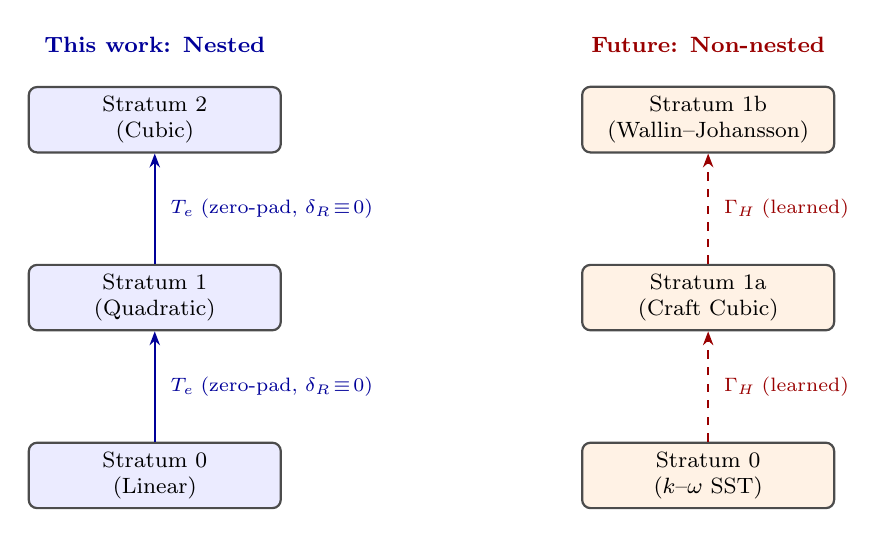
\begin{tikzpicture}[
    node distance=1.4cm and 3.2cm,
    stratum/.style={
      rectangle, rounded corners=3pt, draw=black!70,
      fill=blue!8, minimum width=3.2cm, minimum height=0.7cm,
      font=\footnotesize, align=center, thick
    },
    stratum2/.style={
      rectangle, rounded corners=3pt, draw=black!70,
      fill=orange!10, minimum width=3.2cm, minimum height=0.7cm,
      font=\footnotesize, align=center, thick
    },
    edge_exact/.style={
      -{Stealth[length=5pt]}, thick, blue!60!black
    },
    edge_learned/.style={
      -{Stealth[length=5pt]}, thick, red!60!black, dashed
    },
    label_style/.style={
      font=\scriptsize, midway
    }
  ]
  % --- This work: Vertical (left column) ---
  \node[stratum] (S0L) {Stratum~0\\(Linear)};
  \node[stratum, above=of S0L] (S1L) {Stratum~1\\(Quadratic)};
  \node[stratum, above=of S1L] (S2L) {Stratum~2\\(Cubic)};

  \draw[edge_exact] (S0L) -- (S1L)
    node[label_style, right=2pt] {$T_e$\;(zero-pad, $\dR\!\equiv\!0$)};
  \draw[edge_exact] (S1L) -- (S2L)
    node[label_style, right=2pt] {$T_e$\;(zero-pad, $\dR\!\equiv\!0$)};

  \node[above=0.3cm of S2L, font=\footnotesize\bfseries, blue!60!black]
    {This work: Nested};

  % --- Future: Horizontal (right column) ---
  \node[stratum2, right=3.8cm of S0L] (S0R) {Stratum~0\\($k$--$\omega$ SST)};
  \node[stratum2, above=of S0R] (S1aR) {Stratum~1a\\(Craft Cubic)};
  \node[stratum2, above=of S1aR] (S1bR) {Stratum~1b\\(Wallin--Johansson)};

  \draw[edge_learned] (S0R) -- (S1aR)
    node[label_style, right=2pt] {$\Gamma_H$\;(learned)};
  \draw[edge_learned] (S1aR) -- (S1bR)
    node[label_style, right=2pt] {$\Gamma_H$\;(learned)};

  \node[above=0.3cm of S1bR, font=\footnotesize\bfseries, red!60!black]
    {Future: Non-nested};
\end{tikzpicture}
\caption{Nested vs.\ non-nested structural edits. This work studies
  vertical inclusions where zero-padding is exact by construction.
  The geometric framework becomes non-trivial for horizontal edits
  (basis swaps, model family transitions) where transport maps $\Gamma_H$
  must be learned and path-dependence requires non-convex
  losses.}\label{fig:horizon}
\end{figure}

\subsection{Summary of Contributions}\label{sec:contributions}

\begin{enumerate}
  \item Proposed a geometric framework (Stratified Design Atlas) for
    organizing turbulence closure model families, and demonstrated its
    simplest instantiation---nested constant-coefficient Pope subspaces
    with zero-padding embeddings---in a controlled \emph{a~priori} study.
  \item Quantified the stress-representability gap between linear and
    quadratic Pope strata, recovering the classical Speziale~\cite{Speziale1987}
    result that linear closures produce anti-aligned secondary vorticity
    forcing ($\rho = -0.157$, $29.38\%$ reversed).
  \item Demonstrated that staged calibration relocates transient
    realizability violations into a discardable scaffold stratum, yielding
    essentially monotone deployment dynamics.
  \item Through a $2\times 2$ ablation matrix, identified the transient
    instability mechanism as Adam momentum overshoot, not Gram matrix
    ill-conditioning. The raw basis's scale disparity implicitly
    regularizes Adam's step on $\theta_3$; unit-normalizing
    removes this regularization and increases peak violation from
    $2.0\%$ to $21.8\%$.
  \item A cold-start baseline ($\theta = 0$) contextualizes the
    warm-starting advantage: it converges to the same endpoint with lower
    peak violation, showing that staging benefits are specific to
    momentum-based optimizers.
\end{enumerate}

% ============================================================================
\begin{acknowledgments}
The authors thank the contributors to the NumPy, SciPy, and Matplotlib
projects, whose open-source software made this work possible.
\end{acknowledgments}
% ============================================================================

\paragraph*{Data and Code Availability.}
All source code, experiment scripts, committed telemetry data
(\texttt{results\_curvature\_experiment.json},
\texttt{results\_audit\_experiments.json}), and publication figures
are available in the public repository at
\url{https://github.com/okuhlemadondo/OpDiscovery-FluidMech}.
Every numerical value reported in this paper can be reproduced from the
committed database using the provided scripts.

\begin{thebibliography}{9}

\bibitem{Boussinesq1877}
  J.~Boussinesq,
  \emph{Essai sur la th\'eorie des eaux courantes},
  M\'emoires pr\'esent\'es par divers savants \`a l'Acad\'emie des Sciences
  de l'Institut National de France \textbf{23}(1), 1--680 (1877).

\bibitem{Craft1996}
  T.~J.~Craft, B.~E.~Launder, and K.~Suga,
  \emph{Development and application of a cubic eddy-viscosity model of
    turbulence},
  Int.\ J.\ Heat Fluid Flow \textbf{17}(2), 108--115 (1996).

\bibitem{Lumley1978}
  J.~L.~Lumley,
  \emph{Computational modeling of turbulent flows},
  Adv.\ Appl.\ Mech.\ \textbf{18}, 123--176 (1978).

\bibitem{Pinelli2010}
  A.~Pinelli, M.~Uhlmann, A.~Sekimoto, and G.~Kawahara,
  \emph{Reynolds number dependence of mean flow and turbulence statistics in a
    square duct},
  J.\ Fluid Mech.\ \textbf{644}, 107--122 (2010).

\bibitem{Pope1975}
  S.~B.~Pope,
  \emph{A more general effective-viscosity hypothesis},
  J.\ Fluid Mech.\ \textbf{72}(2), 331--340 (1975).

\bibitem{Prandtl1926}
  L.~Prandtl,
  \emph{\"Uber die ausgebildete Turbulenz},
  Verh.\ 2.\ Int.\ Kongr.\ Tech.\ Mech., Z\"urich, 62--74 (1926).

\bibitem{Schumann1977}
  U.~Schumann,
  \emph{Realizability of Reynolds stress turbulence models},
  Phys.\ Fluids \textbf{20}(5), 721--725 (1977).

\bibitem{Speziale1987}
  C.~G.~Speziale,
  \emph{On nonlinear K-l and K-$\varepsilon$ models of turbulence},
  J.\ Fluid Mech.\ \textbf{178}, 459--475 (1987).

\bibitem{Wallin2000}
  S.~Wallin and A.~V.~Johansson,
  \emph{An explicit algebraic Reynolds stress model for incompressible and
    compressible turbulent flows},
  J.\ Fluid Mech.\ \textbf{403}, 89--132 (2000).

\end{thebibliography}

\end{document}
